\documentclass[/home/jesse/Analysis/FemtoAnalysis/AnalysisNotes/AnalysisNoteJBuxton.tex]{subfiles}
\begin{document}

\subsection{Non-femtoscopic background}
\label{NonFlatBackground}

We observe a significant non-femtoscopic, non-flat, background in all of our correlations at large $k^{*}$.  
This background increases with decreasing centrality, is the same amongst all \LamKpm pairs, and is more pronounced in the \LamKs system, as can be seen in Fig. \ref{fig:CompareAllBgds}.  
Figure \ref{fig:BgdswTHERMK0sTweak:a} shows that THERMINATOR 2 simulation does a good job of describing the difference in backgrounds between \LamKpm and \LamKs.

Before beginning, it is important to note that the difference in \LamKpm and \LamKs backgrounds is due mainly to the difference in kinematic cuts, not due to any interesting physics.  
Figure \ref{fig:BgdswTHERMK0sTweak:b} shows that, for THERMINATOR simulation, when restrictions are imposed on the $p_{\textrm{T}}$ of the \Ks to more closely match the \Kpm cuts, the backgrounds align much better.  
Therefore, we conclude that the difference in background between \LamKpm and \LamKs observed in our experimental data is simply due to a difference in kinematic cuts between \Kpm and \Ks particles.

\begin{figure}[h]
  \centering
  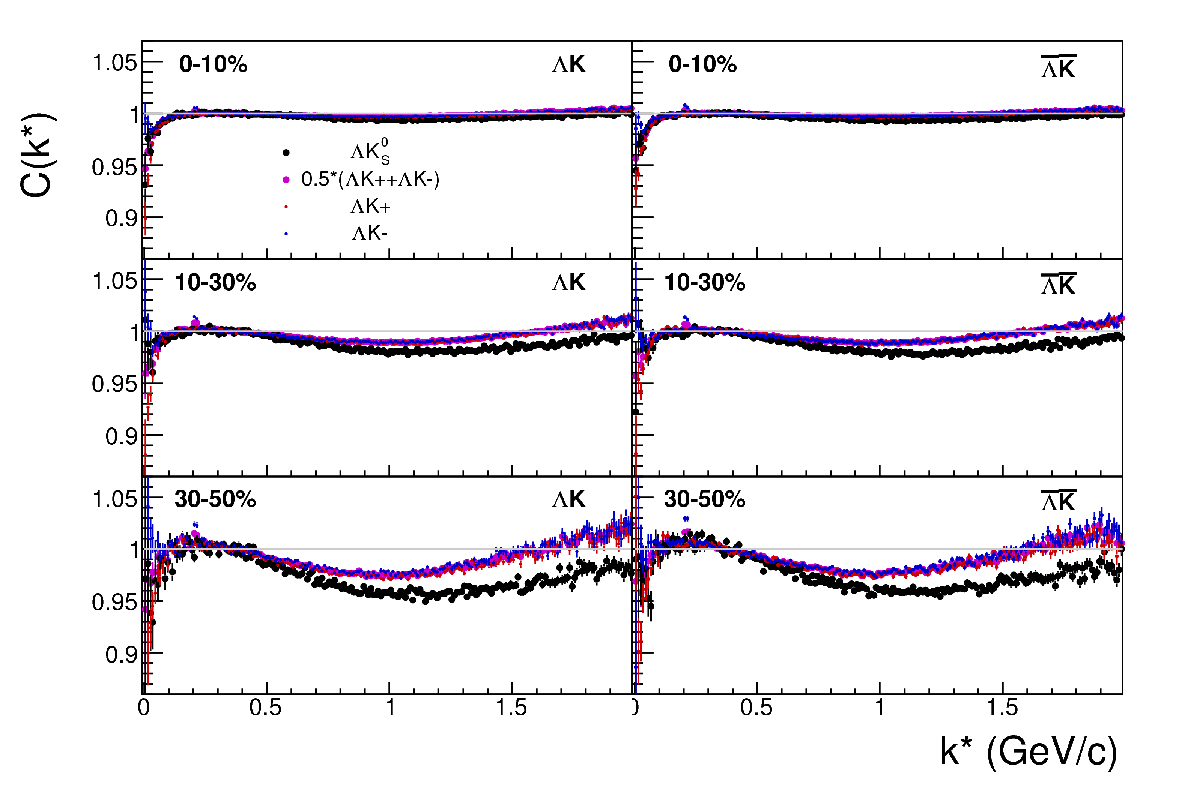
\includegraphics[width=\textwidth]{5_Fitting/Figures/CompareLamKchAvgToLamK0_wIndivKch_0010_1030_3050.pdf}
  \caption[Compare Non-Femtoscopic Backgrounds]{A comparison on the non-femtoscopic backgrounds observed in our our \LamK experimental data.}
  \label{fig:CompareAllBgds}
\end{figure}



\begin{figure}[h!]
  \centering
  %%----start of first subfigure---  
  \subfloat[THERMINATOR standard results]{
    \label{fig:BgdswTHERMK0sTweak:a}
    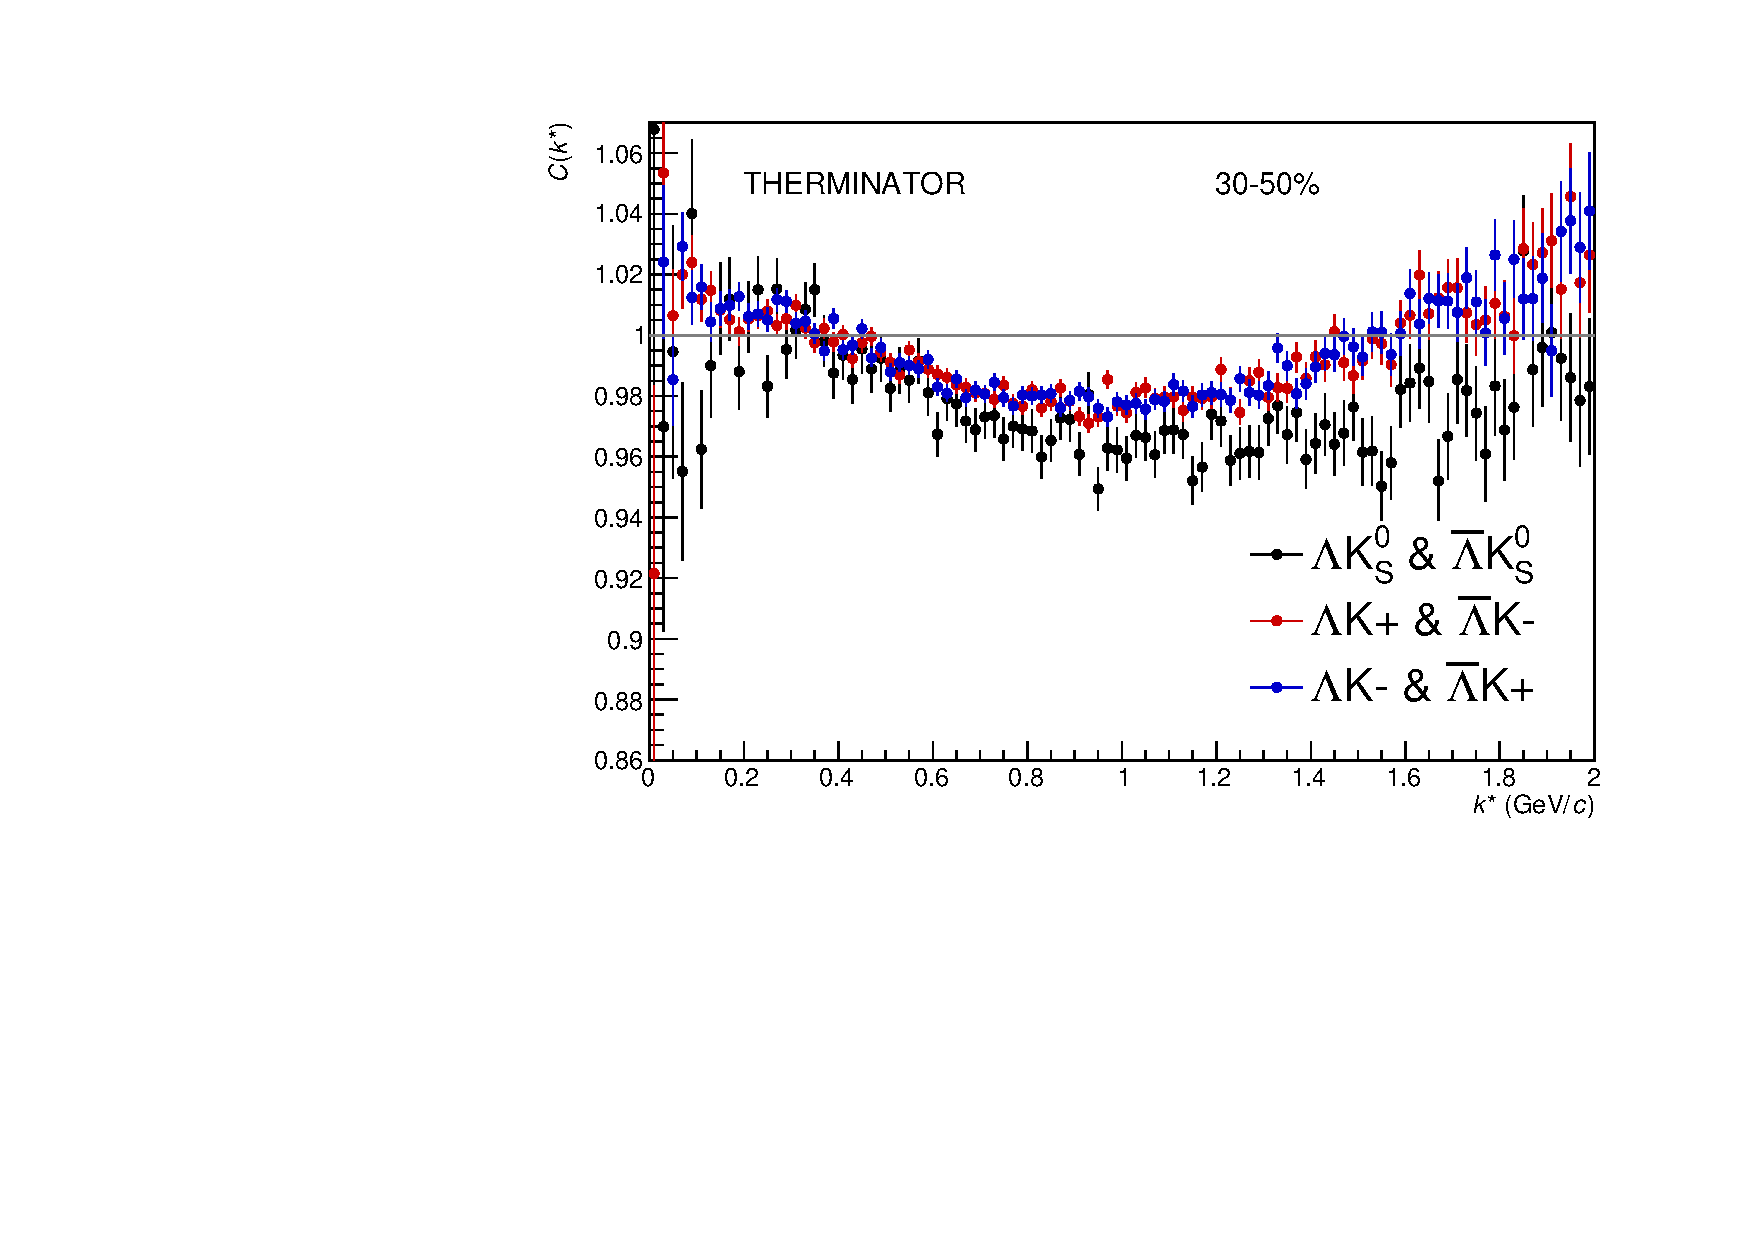
\includegraphics[width=0.49\textwidth]{5_Fitting/Figures/CompareAnalyses_PrimaryOnly_RandomEPs_NumWeight1_PrimaryOnly_wConj_3050.pdf}}
  %%----start of second subfigure---
  \subfloat[THERMINATOR results after upper-$p_{\mathrm{T}}$ cut placed on \Ks to more closely match \Kpm]{
    \label{fig:BgdswTHERMK0sTweak:b}
    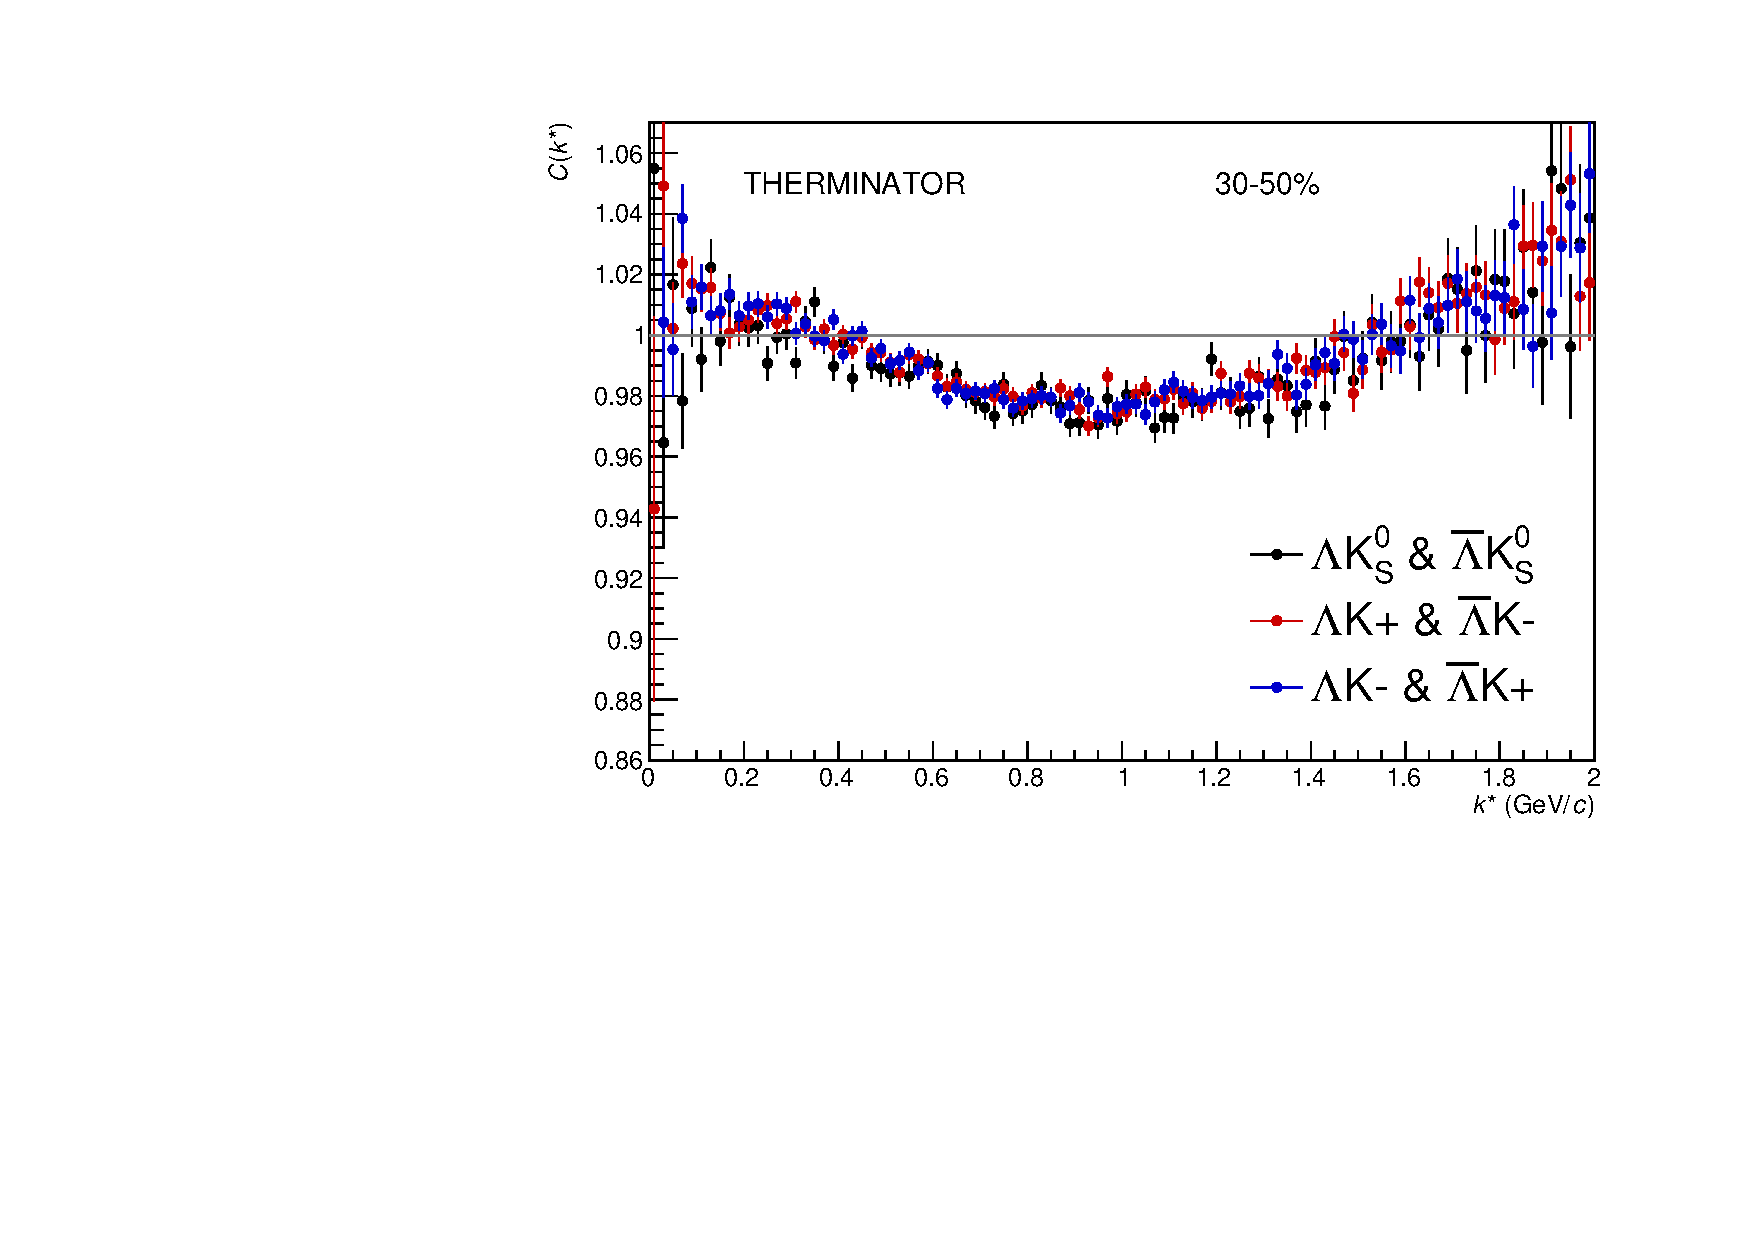
\includegraphics[width=0.49\textwidth]{5_Fitting/Figures/CompareAnalyses_PrimaryOnly_K0sTweak_RandomEPs_NumWeight1_PrimaryOnly_wConj_3050.pdf}}
  %%----overall caption----
  \caption[Backgrounds with THERMINATOR, \Ks Tweak]{THERMINATOR 2 simulation for \LamKchP (red), \LamKchM (blue), and \LamKs (black).  In \ref{fig:BgdswTHERMK0sTweak:a}, we show the standard THERMINATOR 2 results.  THERMINATOR 2 does a good job describing qualitatively the different between the \LamKpm and \LamKs backgrounds.  In \ref{fig:BgdswTHERMK0sTweak:b}, an upper-$p_{\mathrm{T}}$ cut was placed on the \Ks particles to more closely match the \Kpm kinematic cuts.  After this tweak, the \LamKpm and \LamKs backgrounds agree much better.}
  \label{fig:BgdswTHERMK0sTweak}
\end{figure}


It is suggested that this background effect is due primarily to particle collimation associated with elliptic flow \cite{Kisiel:2017}.  
More specifically, these backgrounds result from mixing events with unlike event-plane angles ($\Psi_{\textrm{EP}}$).  
As explained in \cite{Kisiel:2017}, when elliptic flow is present, all particles are more likely to be emitted in a specific direction (in-plane), as opposed to a perpendicular direction.  
Therefore, the difference in momenta for pairs of particles tends to be smaller, compared to the case of no flow.  
In the case of mixed-event pairs, the two events used do not share an event-plane, and therefore there is no collimation effect in the pairs from flow.  
As a result, pairs with larger momentum are more likely when mixed-events are used (in the denominator of the correlation function), causing the correlation function to dip below unity.  
In general, the observation of the correlation function below unity, at a given \kstar, means it is more probable to find a pair at that $k^{*}$ when the daughters are taken from mixed-events, as compared to when they are taken from the same event.
This same reasoning suggests that the background should lead to an enhancement at low-$k^{*}$.  
The enhancement at high-$k^{*}$ ($k^{*} \gtrsim$ 1.5 GeV/$c$) does not result from the collective flow of the system.  
We are not certain what causes this enhancement, but typical suspects are jet-like correlations and resonance decays.

We can split our correlation functions into three main regions.  
First, the low-$k^{*}$ region ($k^{*} \lesssim 0.3$ GeV/$c$) contains the femtoscopic correlations, as well as a likely enhancement from the background.  
The intermediate-$k^{*}$ region (0.3 $\lesssim k^{*} \lesssim$ 1.5 GeV/$c$) contains a suppression from the background.  
Finally, the high-$k^{*}$ region ($k^{*} \gtrsim$ 1.5 GeV/$c$) contains an enhancement with unknown origin.

The issue here is that we need to know the behavior of the non-femtoscopic background in the low-\kstar region, but we only cleanly observe it in the region further out where there is no femtoscopic signal.
Unfortunately, we cannot simply rotate each event to artificially align their event-planes and rid ourselves of this mixing effect, as our azimuthal angle acceptance is not perfectly uniform, and we have only finite event-plane resolution.
With better resolution, one could simply bin events in $\Psi_{\mathrm{EP}}$ and only mix events within a given bin.
We pursued this direction, and observed a slight decrease in the background; however, going to finer binning, we saw no additional reduction in the background, signaling that we had reached the limits dictated by the resolution.
In the end, we are forced to model the background to include it into our fit.

THERMINATOR 2 simulation has been shown to reproduce the background features in a $\pi$K analysis \cite{Kisiel:2017}.  
After issuing each simulated event a random $\Psi_{\mathrm{EP}}$\footnote{default was for all events to share a common event plane}, we found THERMINATOR 2 did an exceptional job of describing our data.  
Furthermore, the simulation showed the non-femtoscopic background affects the correlation function as a separable scale factor (Fig \ref{fig:THERMCfBgdDecomposition}, discussed below).
Figure \ref{fig:BgdswTHERM} shows the THERMINATOR 2 simulation (gold) together with experimental data (red, blue, or black).  
The figure also shows a 6$^{th}$-order polynomial fit to the simulation (gold), as well as the fit polynomial scaled to match the data (red, blue, black).


\begin{figure}[h]
  \centering
  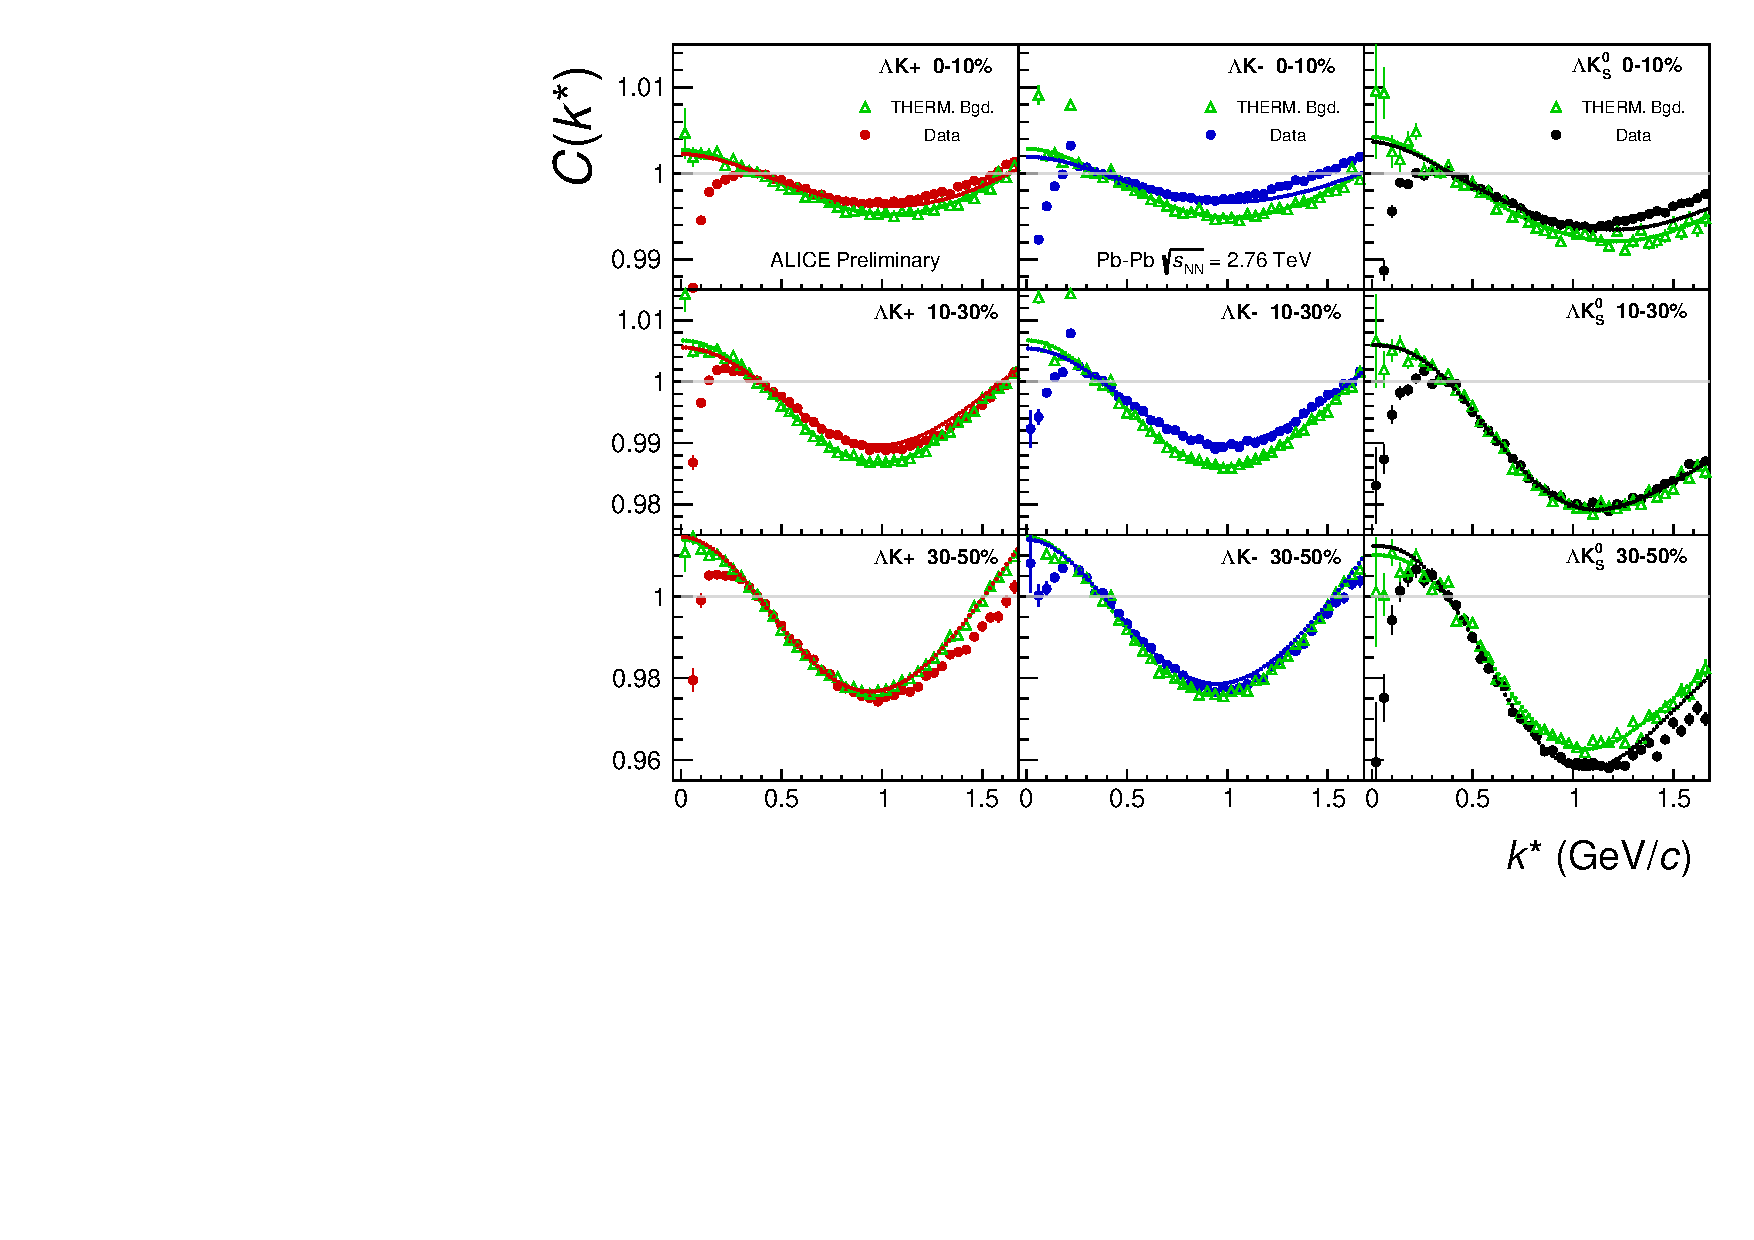
\includegraphics[width=\textwidth]{/home/jesse/Analysis/FemtoAnalysis/AnalysisNotes/5_Fitting/5.5_NonFlatBackground/Figures/BgdwFitOnly_RandomEPs_NumWeight1_Full_AllAnwConj_1030_3050.pdf}
  \caption[Backgrounds with THERMINATOR 2]
  {
  THERMINATOR 2 simulation (gold) together with experimental data (red, blue, or black).  
  Results are shown for \LamKchP (left), \LamKchM (middle), and \LamKs (right).
  A 6$^{th}$-order polynomial fit to the simulation is shown as a solid gold line.  
  This polynomial is scaled to match the experimental data.  
  The polynomial fit with scale factor applied is drawn in a color matching the experimental data (red, blue, black).
  }
  \label{fig:BgdswTHERM}
\end{figure} 

Figure \ref{fig:THERMCfBgdDecomposition} shows three different correlation function generated using THERMINATOR 2 simulation (``Cf w/o Bgd (A)'', ``Cf w. Bgd (B)'', ``Bgd(C)''), as well as two histograms describing the relation between the three (``Ratio (B/C)'', ``1+Diff(B-C)'').  
``Cf w/o Bgd (A)'' shows a correlation function with a femtoscopic correlation, but without background.  
When THERMINATOR 2 is run without randomizing event planes, and therefore having all events share a common event plane, no background is observed, as expected.  
The femtoscopic correlation effect was introduced by assuming a set of scattering parameters for the system, and weighting the numerators appropriately.  
The second correlation, "Cf w. Bgd (B)", shows a correlation function with both a femtoscopic correlation and a background (most closely matches our situation in experiment).  
To generate the background, each event was given a random event-plane angle, as is given to us in experiment.  
To generate the femtoscopic correlation, the same numerator weighting procedure was used.  
Finally, "Bgd (C)", shows a correlation function with a non-femtoscopic background, but no femtoscopic correlation, i.e. background only.  
This is generated just as "Cf w. Bgd (B)", with randomized event planes, but unit weights are used when filling the numerators, so no femtoscopic effects are included.


\begin{figure}[h]
  \centering
  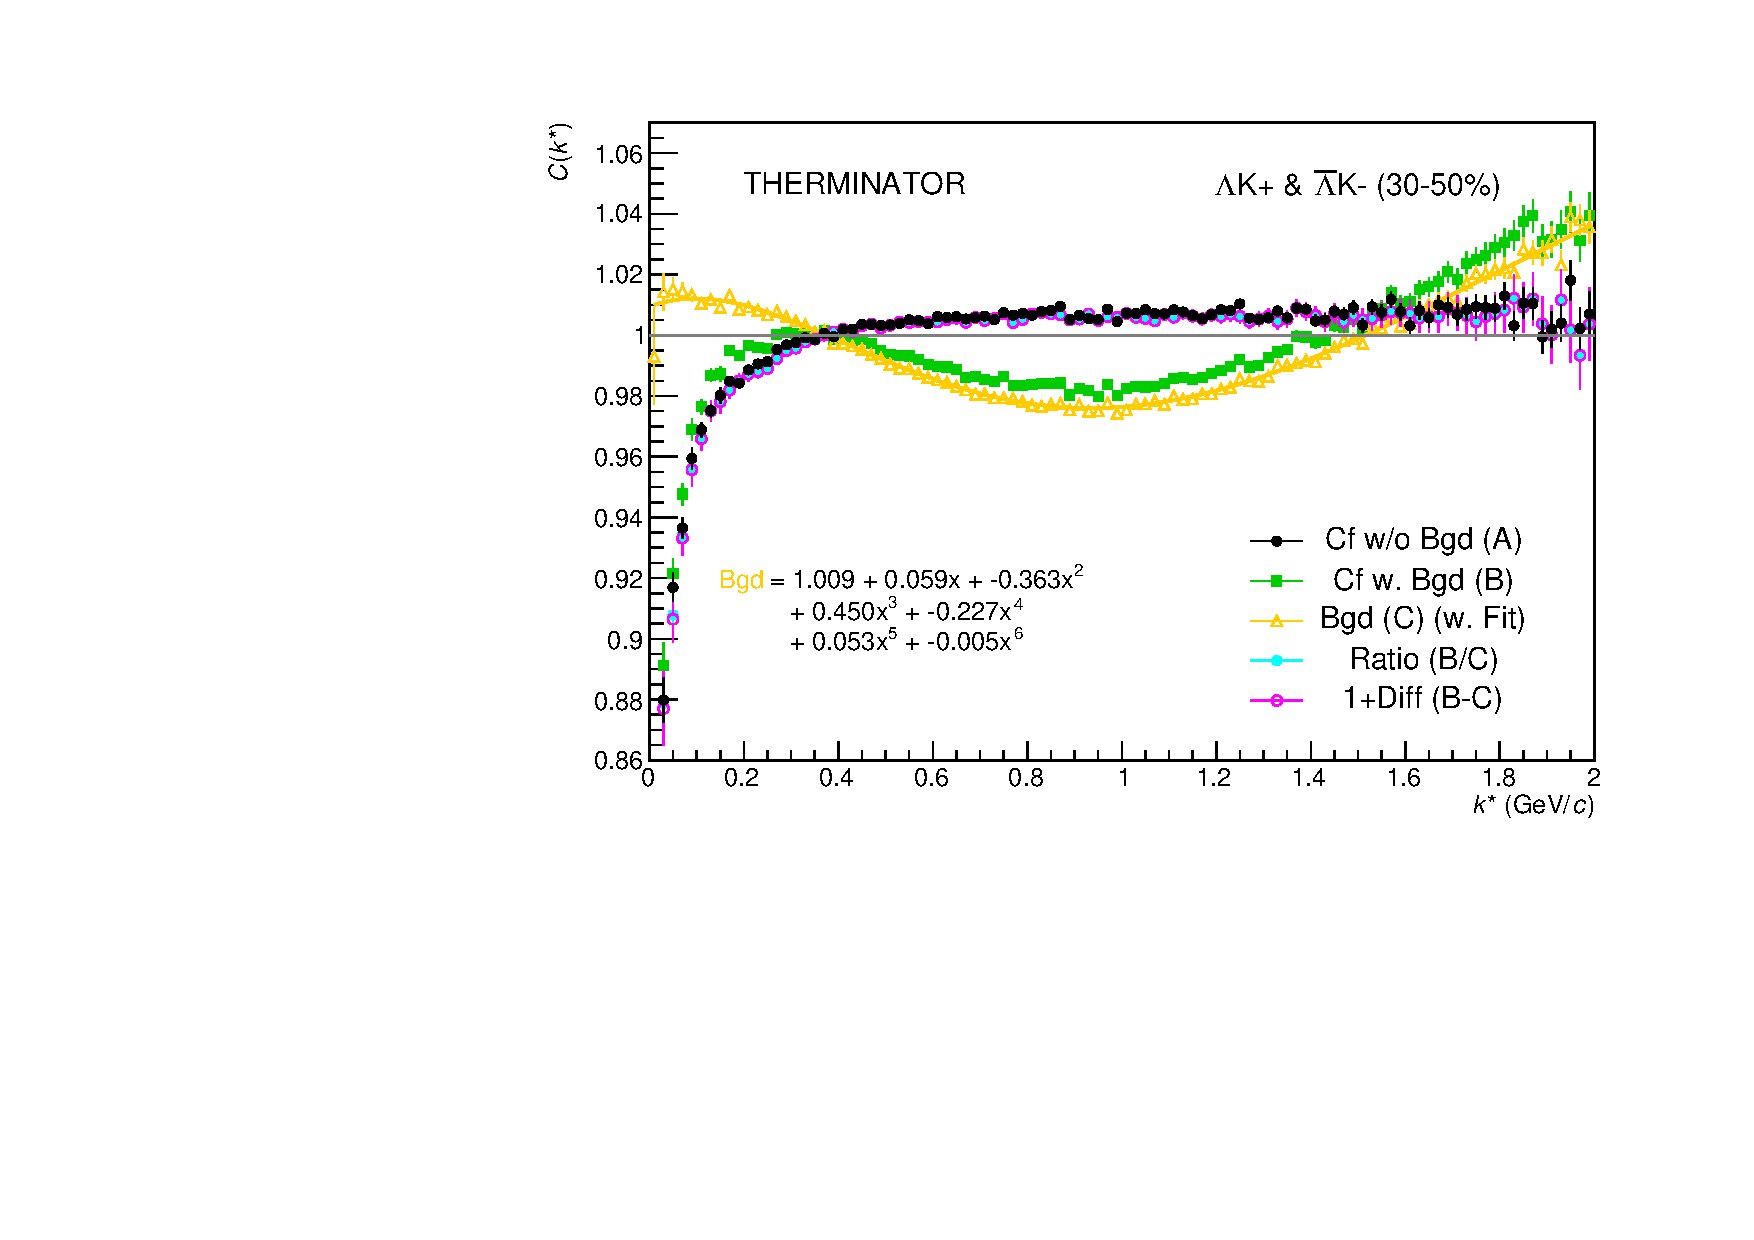
\includegraphics[width=\textwidth]{5_Fitting/Figures/CompareBgds_Full_LamKchPwConj_3050.pdf}
  \caption[Correlation with background decomposition (THERM)]{Correlation with background decomposition with THERMINATOR.  "Cf w/o Bgd (A)" shows a correlation function with a femtoscopic correlation, but without background.  "Cf w. Bgd (B)", shows a correlation function with both a femtoscopic correlation and a background (most closely matches our situation in experiment).  "Bgd (C)", shows a correlation function with a non-femtoscopic background, but no femtoscopic correlation, i.e. background only.}
  \label{fig:THERMCfBgdDecomposition}
\end{figure}


The main point of Fig. \ref{fig:THERMCfBgdDecomposition} is that the black points match the blue (and purple) points; or, equivalently:

\begin{equation}
  Cf w/o Bgd = \dfrac{Cf w. Bgd}{Bgd} \to C_{theory} = \dfrac{C_{exp}}{F_{Bgd}} \to C_{exp} = C_{theory}\cdot F_{Bgd}
  \label{eq:BgdDecomp}
\end{equation}
i.e. THERMINATOR 2 simulation shows the non-femtoscopic background affects the correlation function as a separable scale factor.  
We expect this behavior to be roughly the same in the experimental data.

The description by THERMINATOR 2 of the non-femtoscopic backgrounds in the \LamKpm systems is remarkable, and can be used in a quantitative fashion to help fit the data.
More specifically, the non-femtoscopic backgrounds were modeled by (6$^{\mathrm{th}}$-)order polynomial fits to THERMINATOR 2 simulation for the \LamKpm analyses; one polynomial for each centrality class.
The form of each polynomial was set before use with the experimental data, by fitting to the THERMINATOR 2 simulation, shown in Fig. \ref{fig:BgdswTHERM}.
At the time of the fit, the polynomial used to correct each correlation function could only be adjust by a simple scale factor to best match the data.

The description of the \LamKs is good at a qualitative level, but not quantitatively good enough to be utilized in our fit.
As such, we use a linear form to model the background in the \LamKs system.
The background for each correlation function was fixed before use in the signal region by fitting a linear form to the region $0.6 < k^{*} < 0.9$ GeV/$c$.
In all cases, the non-femtoscopic background correction was applied as a scale factor.

An alternative approach to treating the non-femtoscopic background is to instead attempt to eliminate it.
The background may be effectively reduced by forming the reference distribution ($B(k^{*})$) with the ``Stavinskiy method".
With the Stavinskiy method, mixed-event pairs are not used for the reference distribution; instead, same-event pseudo-pairs, formed by rotating one particle in a real pair by 180$^\circ$ in the transverse plane, are used.  
This rotation rids the pairs of any femtoscopic correlation, while maintaining correlations due to elliptic flow (and other suitably symmetric contributors).
The effect on our \LamK correlation functions can be seen in the appendix, in Sec. \ref{StavCfConstruction}.

Figure \ref{fig:BgdRedMethodsTHERM} demonstrates the use of the Stavinskiy method with THERMINATOR 2.  
In the figure, unit weights were used for all numerators, so no femtoscopic signal is included, only background effects.  
The black points show an ideal, experimentally unreachable, situation of aligning all of the event-plane angles.  
With THERMINATOR 2, when the event-planes are aligned, the background signal is killed.  
The green points show the case of random event-plane angles, a situation more closely matching that of experiment.  
The purple points shown the affect of applying the Stavinskiy method to the case of random event-planes.  
The figure shows that this method effectively kills the non-flat background (i.e. the procedure takes the green points to the purple).  
Finally, the blue points show the effect of applying the Stavinskiy method when all of the event-planes are aligned.  
This shows that the Stavinskiy method does not introduce any signal to an already flat background.


\begin{figure}[h]
  \centering
  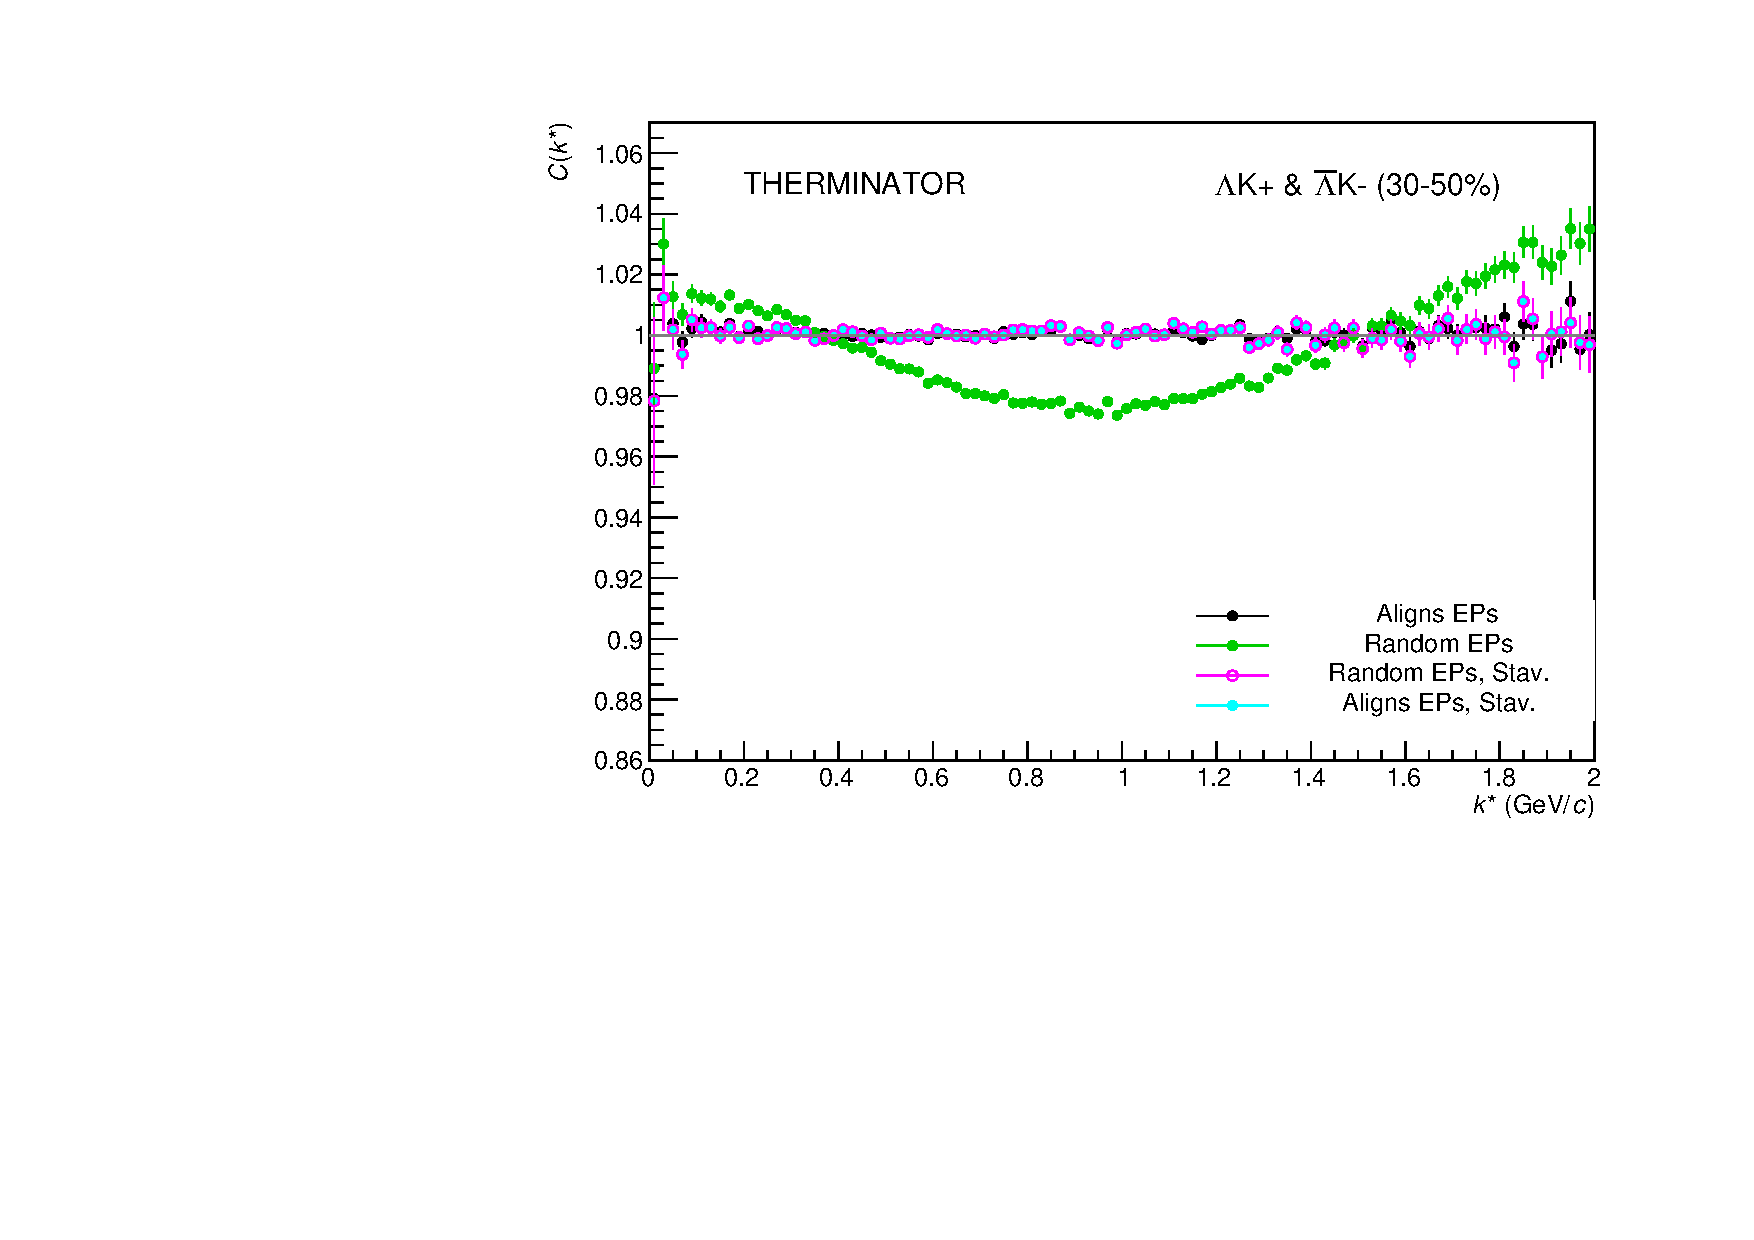
\includegraphics[width=\textwidth]{5_Fitting/Figures/CompareBackgroundReductionMethods_Full_LamKchPwConj_3050_NumWeight1.pdf}
  \caption[Background reduction methods with THERMINATOR]{The use of the Stavinskiy method with THERMINATOR 2.  Unit weights were used for all numerators, so no femtoscopic signal is included, only background effects.  The black points show an ideal, experimentally unreachable, situation of aligning all of the event-plane angles.  The green points show the experimental situation of random event-plane angles.  The purple points shown the affect of applying the Stavinskiy method to the case of random event-planes.  Finally, the blue points show the effect of applying the Stavinskiy method when all of the event-planes are aligned.}
  \label{fig:BgdRedMethodsTHERM}
\end{figure}








\end{document}